\documentclass[letterpaper,headings=standardclasses]{scrartcl}

\usepackage[margin=1in,includefoot]{geometry}
\usepackage{amssymb}
\usepackage{amsmath}
\usepackage{listings}
\usepackage{tikz}
\usepackage{float}

\usetikzlibrary{shapes,arrows}

\tikzset{
  block/.style    = {draw, thick, rectangle, minimum height = 3em, minimum width = 3em},
  sum/.style      = {draw, circle},
  input/.style    = {coordinate, circle},
  output/.style   = {coordinate, circle}
}

\lstset{basicstyle=\ttfamily,language=python,columns=flexible,breaklines=true,showstringspaces=false}

\title{Homework 6}
\subtitle{CS 559 - Neural Networks - Fall 2019}
\author{Matteo Corain 650088272}

\begin{document}

\maketitle

\section{Question 1}

\subsection{Generation of patterns and weights}

The first step that has been taken for the solution of this problem has been to generate all the patterns represented by sequences of $\pm 1$ with length $m$ (in the considered case, $m = 4$ has been used). For this purpose, the recursive function \texttt{gen\_patterns()} has been used, which generates the dispositions with replacement of the two values on a vector of length $m$. This function receives the vector $x$ to be used, the position to be filled for the current recursive call, the length $m$ of the vector and the array of patterns to be returned, and performs the following actions:

\begin{itemize}
    \item It checks whether the $x$ vector has already been filled or not (\texttt{pos == m}), in which case it appends the generated pattern to the list of patterns and returns it;
    \item Otherwise, it proceeds to set the \texttt{pos}-th value of the vector first to -1 and then to 1, each time recursively calling itself on the successive position.
\end{itemize}

Once that all pattern combinations have been computed, $n$ independent samples are chosen to be stored in the network (in our case, $n = 5$ was chosen). For this purpose, the array of pattern is randomly shuffled, then a loop is started (running until the length of the list of selected samples reaches the value of $n$), checking whether each pattern $x$ (or its opposite $-x$) has already been chosen for the purpose and, if not, adding it to the list of selected samples.

Having set the random seed to a fixed value for reproducibility of the results, the following patterns have been generated for storage:

$$ x_1 = \left[\begin{matrix} -1 \\ -1 \\ -1 \\ -1 \end{matrix}\right], x_2 = \left[\begin{matrix} -1 \\ -1 \\ -1 \\ +1 \end{matrix}\right], x_3 = \left[\begin{matrix} -1 \\ -1 \\ +1 \\ -1 \end{matrix}\right], x_4 = \left[\begin{matrix} -1 \\ -1 \\ +1 \\ +1 \end{matrix}\right], x_5 = \left[\begin{matrix} -1 \\ +1 \\ +1 \\ -1 \end{matrix}\right] $$

Starting from those patterns, the weight matrix for the network has been generated using the standard approach, obtaining the following result:

$$ W = \sum_{i =+1}^n x_i x_i^T = \left[ \begin{matrix}
    +5 & +3 & -1 & +1 \\
    +3 & +5 & +1 & -1 \\
    -1 & +1 & +5 & -1 \\
    +1 & -1 & -1 & +5
\end{matrix} \right] $$

\subsection{Search of spurious patterns}

For the search of spurious patterns, the \texttt{spurious\_search()} has been introduced, which takes as arguments the list of all patterns, the list of selected samples and the weight matrix. For each pattern $z$, it checks whether $z$ or $-z$ were chosen for storage and, in case they were not, if they are effectively spurious patterns, meaning that:

$$ z = \phi(Wz), z \notin \{x_i\} $$

All spurious patterns are collected in a list that is finally returned. For the described case, the following spurious patterns have been identified:

$$ z_1 = \left[\begin{matrix} -1 \\ +1 \\ -1 \\ -1 \end{matrix}\right], z_2 = \left[\begin{matrix} -1 \\ +1 \\ +1 \\ +1 \end{matrix}\right], z_3 = \left[\begin{matrix} +1 \\ -1 \\ -1 \\ -1 \end{matrix}\right], z_4 = \left[\begin{matrix} +1 \\ -1 \\ +1 \\ +1 \end{matrix}\right] $$

\subsection{Complete Python code}

\lstinputlisting[basicstyle=\ttfamily\scriptsize]{hw6_ex1.py}

\section{Question 2}

\subsection{Network representation}

The proposed Hopfield network is characterized by the following parameters:

\begin{itemize}
    \item Biases $\theta_0 = \theta_1 = \theta_2 = 0.5$;
    \item Weights $w_{12} = w_{21} = 2$;
    \item Weights $w_{13} = w_{31} = -1$;
    \item Weights $w_{23} = w_{32} = -1$;
    \item Weights $w_{11} = w_{22} = 0$;
    \item Weight $w_{33} = 1$.
\end{itemize}

Where neuron 1 indicates the topmost in the figure, neuron 2 the leftmost and neuron 3 the rightmost. These features may be formalized in a matrix form as:

$$ \theta = \left[ \begin{matrix} \theta_1 \\ \theta_2 \\ \theta_3 \end{matrix} \right] = \left[ \begin{matrix} 0.5 \\ 0.5 \\ 0.5 \end{matrix} \right], W = \left[ \begin{matrix} w_{11} & w_{12} & w_{13} \\ w_{21} & w_{22} & w_{23} \\ w_{31} & w_{32} & w_{33} \end{matrix} \right] = \left[ \begin{matrix} 0 & 2 & -1 \\ 2 & 0 & -1 \\ -1 & -1 & 1 \end{matrix} \right] $$

\subsection{State energy computation}

Given these two matrices, for each state $x$ of the network the energy associated with that state is defined by:

$$ E(x) = - x^T W x - 2 x^T \theta $$

Applying the presented formula to each of the possible $2^n = 2^3 = 8$ states in which the considered network can be, we obtain the results in table \ref{entable}.

\begin{table}[h]
    \centering
    \begin{tabular}{|c|c|c|c|}
    \hline
    $x_1$ & $x_2$ & $x_3$ & $E(x)$ \\ \hline
    -1 & -1 & -1 & +2 \\ \hline
    -1 & -1 & +1 & -8 \\ \hline
    -1 & +1 & -1 & +4 \\ \hline
    -1 & +1 & +1 & +2 \\ \hline
    +1 & -1 & -1 & +4 \\ \hline
    +1 & -1 & +1 & +2 \\ \hline
    +1 & +1 & -1 & -10 \\ \hline
    +1 & +1 & +1 & -4 \\ \hline
    \end{tabular}
    \caption{Energy of each network state}
    \label{entable}
\end{table}

\subsection{Synchronous update}

In the context of Hopfield networks, synchronous update prescribes that all the components of the state $x$ of the considered network are updated at once, according to the update rule:

$$ x \leftarrow \phi(Wx + \theta) $$

Where $W$ is the weight matrix of the network and $\theta$ the bias vector. Applying the aforementioned update rule to each possible state of the network, it is possible to compute the successor state for each possible state of the network. Derivations are shown below:

\begin{itemize}
    \item $x = [\begin{matrix} -1 & -1 & -1 \end{matrix}]^T$:
    
    $$ x' = \phi(Wx + \theta) = \phi \left( \left[ \begin{matrix} 0 & 2 & -1 \\ 2 & 0 & -1 \\ -1 & -1 & 1 \end{matrix} \right] \left[ \begin{matrix} -1 \\ -1 \\ -1 \end{matrix} \right] + \left[ \begin{matrix} 0.5 \\ 0.5 \\ 0.5 \end{matrix} \right] \right) = \phi \left( \left[ \begin{matrix} -0.5 \\ -0.5 \\ +1.5 \end{matrix} \right] \right) = \left[ \begin{matrix} -1 \\ -1 \\ +1 \end{matrix} \right] $$

    \item $x = [\begin{matrix} -1 & -1 & +1 \end{matrix}]^T$:
    
    $$ x' = \phi(Wx + \theta) = \phi \left( \left[ \begin{matrix} 0 & 2 & -1 \\ 2 & 0 & -1 \\ -1 & -1 & 1 \end{matrix} \right] \left[ \begin{matrix} -1 \\ -1 \\ +1 \end{matrix} \right] + \left[ \begin{matrix} 0.5 \\ 0.5 \\ 0.5 \end{matrix} \right] \right) = \phi \left( \left[ \begin{matrix} -2.5 \\ -2.5 \\ +3.5 \end{matrix} \right] \right) = \left[ \begin{matrix} -1 \\ -1 \\ +1 \end{matrix} \right] $$

    \item $x = [\begin{matrix} -1 & +1 & -1 \end{matrix}]^T$:
    
    $$ x' = \phi(Wx + \theta) = \phi \left( \left[ \begin{matrix} 0 & 2 & -1 \\ 2 & 0 & -1 \\ -1 & -1 & 1 \end{matrix} \right] \left[ \begin{matrix} -1 \\ +1 \\ -1 \end{matrix} \right] + \left[ \begin{matrix} 0.5 \\ 0.5 \\ 0.5 \end{matrix} \right] \right) = \phi \left( \left[ \begin{matrix} +3.5 \\ -0.5 \\ -0.5 \end{matrix} \right] \right) = \left[ \begin{matrix} +1 \\ -1 \\ -1 \end{matrix} \right] $$

    \item $x = [\begin{matrix} -1 & +1 & +1 \end{matrix}]^T$:
    
    $$ x' = \phi(Wx + \theta) = \phi \left( \left[ \begin{matrix} 0 & 2 & -1 \\ 2 & 0 & -1 \\ -1 & -1 & 1 \end{matrix} \right] \left[ \begin{matrix} -1 \\ +1 \\ +1 \end{matrix} \right] + \left[ \begin{matrix} 0.5 \\ 0.5 \\ 0.5 \end{matrix} \right] \right) = \phi \left( \left[ \begin{matrix} +1.5 \\ -2.5 \\ +1.5 \end{matrix} \right] \right) = \left[ \begin{matrix} +1 \\ -1 \\ +1 \end{matrix} \right] $$

    \item $x = [\begin{matrix} +1 & -1 & -1 \end{matrix}]^T$:
    
    $$ x' = \phi(Wx + \theta) = \phi \left( \left[ \begin{matrix} 0 & 2 & -1 \\ 2 & 0 & -1 \\ -1 & -1 & 1 \end{matrix} \right] \left[ \begin{matrix} +1 \\ -1 \\ -1 \end{matrix} \right] + \left[ \begin{matrix} 0.5 \\ 0.5 \\ 0.5 \end{matrix} \right] \right) = \phi \left( \left[ \begin{matrix} -0.5 \\ +3.5 \\ -0.5 \end{matrix} \right] \right) = \left[ \begin{matrix} -1 \\ +1 \\ -1 \end{matrix} \right] $$

    \item $x = [\begin{matrix} +1 & -1 & +1 \end{matrix}]^T$:
    
    $$ x' = \phi(Wx + \theta) = \phi \left( \left[ \begin{matrix} 0 & 2 & -1 \\ 2 & 0 & -1 \\ -1 & -1 & 1 \end{matrix} \right] \left[ \begin{matrix} +1 \\ -1 \\ +1 \end{matrix} \right] + \left[ \begin{matrix} 0.5 \\ 0.5 \\ 0.5 \end{matrix} \right] \right) = \phi \left( \left[ \begin{matrix} -2.5 \\ +1.5 \\ +1.5 \end{matrix} \right] \right) = \left[ \begin{matrix} -1 \\ +1 \\ +1 \end{matrix} \right] $$

    \item $x = [\begin{matrix} +1 & +1 & -1 \end{matrix}]^T$:
    
    $$ x' = \phi(Wx + \theta) = \phi \left( \left[ \begin{matrix} 0 & 2 & -1 \\ 2 & 0 & -1 \\ -1 & -1 & 1 \end{matrix} \right] \left[ \begin{matrix} +1 \\ +1 \\ -1 \end{matrix} \right] + \left[ \begin{matrix} 0.5 \\ 0.5 \\ 0.5 \end{matrix} \right] \right) = \phi \left( \left[ \begin{matrix} +3.5 \\ +3.5 \\ -3.5 \end{matrix} \right] \right) = \left[ \begin{matrix} +1 \\ +1 \\ -1 \end{matrix} \right] $$
    
    \item $x = [\begin{matrix} +1 & +1 & +1 \end{matrix}]^T$:
    
    $$ x' = \phi(Wx + \theta) = \phi \left( \left[ \begin{matrix} 0 & 2 & -1 \\ 2 & 0 & -1 \\ -1 & -1 & 1 \end{matrix} \right] \left[ \begin{matrix} +1 \\ +1 \\ +1 \end{matrix} \right] + \left[ \begin{matrix} 0.5 \\ 0.5 \\ 0.5 \end{matrix} \right] \right) = \phi \left( \left[ \begin{matrix} +1.5 \\ +1.5 \\ -0.5 \end{matrix} \right] \right) = \left[ \begin{matrix} +1 \\ +1 \\ -1 \end{matrix} \right] $$
\end{itemize}

Similar computations have been performed for all the other states, obtaining the state transition diagram shown in figure \ref{sync}.

\begin{figure}[h]
    \centering
    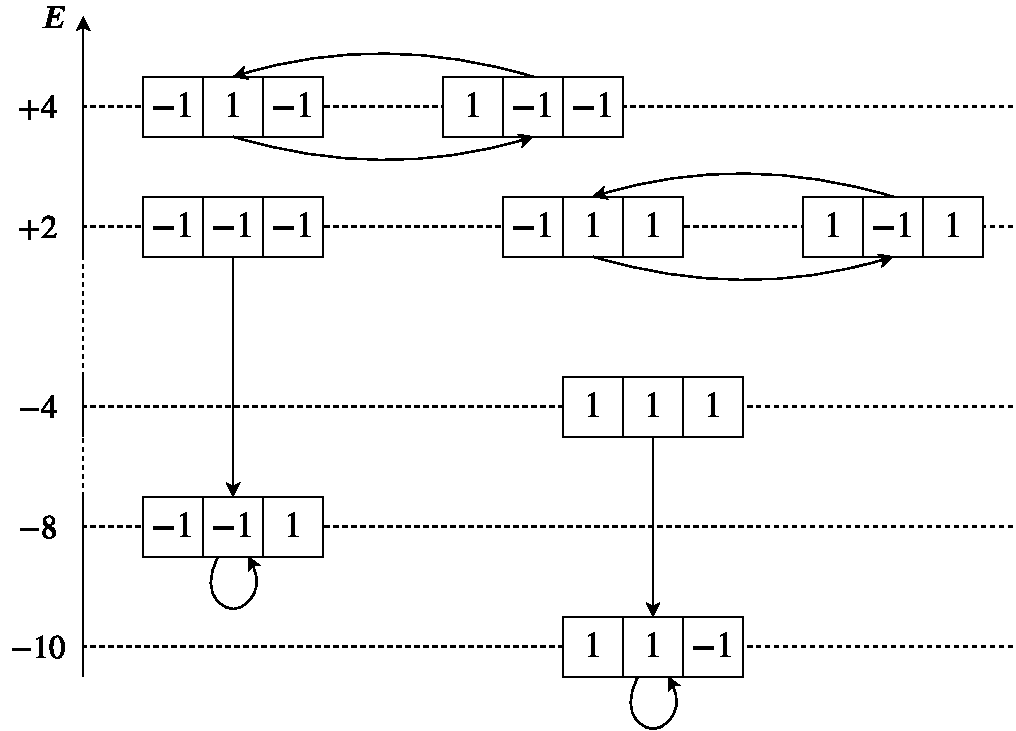
\includegraphics[width=0.7\linewidth]{sync.pdf}
    \caption{State transition diagram with synchronous update}
    \label{sync}
\end{figure}

As it can be seen, this form of update may generate instability, since there are some states that are never able to converge to a stable configuration. In this case, the \emph{urstates} of the network are $[\begin{matrix} -1 & -1 & -1 \end{matrix}]^T$ and $[\begin{matrix} +1 & +1 & +1 \end{matrix}]^T$ (they have no predecessor states, including themselves), while the \emph{stable states} of the network are $[\begin{matrix} -1 & -1 & +1 \end{matrix}]^T$ and $[\begin{matrix} +1 & +1 & -1 \end{matrix}]^T$ (they have no successor states, excluding themselves).

\subsection{Asynchronous update}

In the context of Hopfield networks, asynchronous update prescribes that the components of the state $x$ of the considered network are updated one at a time, fixing the values of the others. In formulas, we have that:

$$ x_i \leftarrow W_i x + \theta_i, i = 1, \dots, m $$

Where $W_i$ denotes the $i$-th row of the weight matrix and $\theta_i$ the $i$-th component of the bias vector. In the case of asynchronous update, therefore, different updates are possible on different components, potentially making the network transition to different states. Derivations in the case of independent update of the single components are shown below:

\begin{itemize}
\item $x = [\begin{matrix} -1 & -1 & -1 \end{matrix}]^T$:

$$ x'_{1} = \phi(W_1 x + \theta_1) = \phi \left( \left[ \begin{matrix} 0 & 2 & -1 \end{matrix} \right] \left[ \begin{matrix} -1 \\ -1 \\ -1 \end{matrix} \right] + 0.5 \right) = \phi \left( -0.5 \right) = -1 \Rightarrow x' = \left[ \begin{matrix} -1 \\ -1 \\ -1 \end{matrix} \right] $$

$$ x'_{2} = \phi(W_2 x + \theta_2) = \phi \left( \left[ \begin{matrix} 2 & 0 & -1 \end{matrix} \right] \left[ \begin{matrix} -1 \\ -1 \\ -1 \end{matrix} \right] + 0.5 \right) = \phi \left( -0.5 \right) = -1 \Rightarrow x' = \left[ \begin{matrix} -1 \\ -1 \\ -1 \end{matrix} \right] $$

$$ x'_{3} = \phi(W_3 x + \theta_3) = \phi \left( \left[ \begin{matrix} -1 & -1 & 1 \end{matrix} \right] \left[ \begin{matrix} -1 \\ -1 \\ -1 \end{matrix} \right] + 0.5 \right) = \phi \left( 1.5 \right) = +1 \Rightarrow x' = \left[ \begin{matrix} -1 \\ -1 \\ +1 \end{matrix} \right] $$

\item $x = [\begin{matrix} -1 & -1 & +1 \end{matrix}]^T$:

$$ x'_{1} = \phi(W_1 x + \theta_1) = \phi \left( \left[ \begin{matrix} 0 & 2 & -1 \end{matrix} \right] \left[ \begin{matrix} -1 \\ -1 \\ +1 \end{matrix} \right] + 0.5 \right) = \phi \left( -2.5 \right) = -1 \Rightarrow x' = \left[ \begin{matrix} -1 \\ -1 \\ +1 \end{matrix} \right] $$

$$ x'_{2} = \phi(W_2 x + \theta_2) = \phi \left( \left[ \begin{matrix} 2 & 0 & -1 \end{matrix} \right] \left[ \begin{matrix} -1 \\ -1 \\ +1 \end{matrix} \right] + 0.5 \right) = \phi \left( -2.5 \right) = -1 \Rightarrow x' = \left[ \begin{matrix} -1 \\ -1 \\ +1 \end{matrix} \right] $$

$$ x'_{3} = \phi(W_3 x + \theta_3) = \phi \left( \left[ \begin{matrix} -1 & -1 & 1 \end{matrix} \right] \left[ \begin{matrix} -1 \\ -1 \\ +1 \end{matrix} \right] + 0.5 \right) = \phi \left( +3.5 \right) = +1 \Rightarrow x' = \left[ \begin{matrix} -1 \\ -1 \\ +1 \end{matrix} \right] $$

\item $x = [\begin{matrix} -1 & +1 & -1 \end{matrix}]^T$:

$$ x'_{1} = \phi(W_1 x + \theta_1) = \phi \left( \left[ \begin{matrix} 0 & 2 & -1 \end{matrix} \right] \left[ \begin{matrix} -1 \\ +1 \\ -1 \end{matrix} \right] + 0.5 \right) = \phi \left( +3.5 \right) = +1 \Rightarrow x' = \left[ \begin{matrix} +1 \\ +1 \\ -1 \end{matrix} \right] $$

$$ x'_{2} = \phi(W_2 x + \theta_2) = \phi \left( \left[ \begin{matrix} 2 & 0 & -1 \end{matrix} \right] \left[ \begin{matrix} -1 \\ +1 \\ -1 \end{matrix} \right] + 0.5 \right) = \phi \left( -0.5 \right) = -1 \Rightarrow x' = \left[ \begin{matrix} -1 \\ -1 \\ -1 \end{matrix} \right] $$

$$ x'_{3} = \phi(W_3 x + \theta_3) = \phi \left( \left[ \begin{matrix} -1 & -1 & 1 \end{matrix} \right] \left[ \begin{matrix} -1 \\ +1 \\ -1 \end{matrix} \right] + 0.5 \right) = \phi \left( -0.5 \right) = -1 \Rightarrow x' = \left[ \begin{matrix} -1 \\ +1 \\ -1 \end{matrix} \right] $$

\item $x = [\begin{matrix} -1 & +1 & +1 \end{matrix}]^T$:

$$ x'_{1} = \phi(W_1 x + \theta_1) = \phi \left( \left[ \begin{matrix} 0 & 2 & -1 \end{matrix} \right] \left[ \begin{matrix} -1 \\ +1 \\ +1 \end{matrix} \right] + 0.5 \right) = \phi \left( +1.5 \right) = +1 \Rightarrow x' = \left[ \begin{matrix} +1 \\ +1 \\ +1 \end{matrix} \right] $$

$$ x'_{2} = \phi(W_2 x + \theta_2) = \phi \left( \left[ \begin{matrix} 2 & 0 & -1 \end{matrix} \right] \left[ \begin{matrix} -1 \\ +1 \\ +1 \end{matrix} \right] + 0.5 \right) = \phi \left( -2.5 \right) = -1 \Rightarrow x' = \left[ \begin{matrix} -1 \\ -1 \\ +1 \end{matrix} \right] $$

$$ x'_{3} = \phi(W_3 x + \theta_3) = \phi \left( \left[ \begin{matrix} -1 & -1 & 1 \end{matrix} \right] \left[ \begin{matrix} -1 \\ +1 \\ +1 \end{matrix} \right] + 0.5 \right) = \phi \left( +1.5 \right) = +1 \Rightarrow x' = \left[ \begin{matrix} -1 \\ +1 \\ +1 \end{matrix} \right] $$

\item $x = [\begin{matrix} +1 & -1 & -1 \end{matrix}]^T$:

$$ x'_{1} = \phi(W_1 x + \theta_1) = \phi \left( \left[ \begin{matrix} 0 & 2 & -1 \end{matrix} \right] \left[ \begin{matrix} +1 \\ -1 \\ -1 \end{matrix} \right] + 0.5 \right) = \phi \left( -0.5 \right) = -1 \Rightarrow x' = \left[ \begin{matrix} -1 \\ -1 \\ -1 \end{matrix} \right] $$

$$ x'_{2} = \phi(W_2 x + \theta_2) = \phi \left( \left[ \begin{matrix} 2 & 0 & -1 \end{matrix} \right] \left[ \begin{matrix} +1 \\ -1 \\ -1 \end{matrix} \right] + 0.5 \right) = \phi \left( +3.5 \right) = +1 \Rightarrow x' = \left[ \begin{matrix} +1 \\ +1 \\ -1 \end{matrix} \right] $$

$$ x'_{3} = \phi(W_3 x + \theta_3) = \phi \left( \left[ \begin{matrix} -1 & -1 & 1 \end{matrix} \right] \left[ \begin{matrix} +1 \\ -1 \\ -1 \end{matrix} \right] + 0.5 \right) = \phi \left( -0.5 \right) = -1 \Rightarrow x' = \left[ \begin{matrix} +1 \\ -1 \\ -1 \end{matrix} \right] $$

\item $x = [\begin{matrix} +1 & -1 & +1 \end{matrix}]^T$:

$$ x'_{1} = \phi(W_1 x + \theta_1) = \phi \left( \left[ \begin{matrix} 0 & 2 & -1 \end{matrix} \right] \left[ \begin{matrix} +1 \\ -1 \\ +1 \end{matrix} \right] + 0.5 \right) = \phi \left( -2.5 \right) = -1 \Rightarrow x' = \left[ \begin{matrix} -1 \\ -1 \\ +1 \end{matrix} \right] $$

$$ x'_{2} = \phi(W_2 x + \theta_2) = \phi \left( \left[ \begin{matrix} 2 & 0 & -1 \end{matrix} \right] \left[ \begin{matrix} +1 \\ -1 \\ +1 \end{matrix} \right] + 0.5 \right) = \phi \left( +1.5 \right) = +1 \Rightarrow x' = \left[ \begin{matrix} +1 \\ +1 \\ +1 \end{matrix} \right] $$

$$ x'_{3} = \phi(W_3 x + \theta_3) = \phi \left( \left[ \begin{matrix} -1 & -1 & 1 \end{matrix} \right] \left[ \begin{matrix} +1 \\ -1 \\ +1 \end{matrix} \right] + 0.5 \right) = \phi \left( +1.5 \right) = +1 \Rightarrow x' = \left[ \begin{matrix} +1 \\ -1 \\ +1 \end{matrix} \right] $$

\item $x = [\begin{matrix} +1 & +1 & -1 \end{matrix}]^T$:

$$ x'_{1} = \phi(W_1 x + \theta_1) = \phi \left( \left[ \begin{matrix} 0 & 2 & -1 \end{matrix} \right] \left[ \begin{matrix} +1 \\ +1 \\ -1 \end{matrix} \right] + 0.5 \right) = \phi \left( +3.5 \right) = +1 \Rightarrow x' = \left[ \begin{matrix} +1 \\ +1 \\ -1 \end{matrix} \right] $$

$$ x'_{2} = \phi(W_2 x + \theta_2) = \phi \left( \left[ \begin{matrix} 2 & 0 & -1 \end{matrix} \right] \left[ \begin{matrix} +1 \\ +1 \\ -1 \end{matrix} \right] + 0.5 \right) = \phi \left( +3.5 \right) = +1 \Rightarrow x' = \left[ \begin{matrix} +1 \\ +1 \\ -1 \end{matrix} \right] $$

$$ x'_{3} = \phi(W_3 x + \theta_3) = \phi \left( \left[ \begin{matrix} -1 & -1 & 1 \end{matrix} \right] \left[ \begin{matrix} +1 \\ +1 \\ -1 \end{matrix} \right] + 0.5 \right) = \phi \left( -3.5 \right) = -1 \Rightarrow x' = \left[ \begin{matrix} +1 \\ +1 \\ -1 \end{matrix} \right] $$

\item $x = [\begin{matrix} +1 & +1 & +1 \end{matrix}]^T$:

$$ x'_{1} = \phi(W_1 x + \theta_1) = \phi \left( \left[ \begin{matrix} 0 & 2 & -1 \end{matrix} \right] \left[ \begin{matrix} +1 \\ +1 \\ +1 \end{matrix} \right] + 0.5 \right) = \phi \left( +1.5 \right) = +1 \Rightarrow x' = \left[ \begin{matrix} +1 \\ +1 \\ +1 \end{matrix} \right] $$

$$ x'_{2} = \phi(W_2 x + \theta_2) = \phi \left( \left[ \begin{matrix} 2 & 0 & -1 \end{matrix} \right] \left[ \begin{matrix} +1 \\ +1 \\ +1 \end{matrix} \right] + 0.5 \right) = \phi \left( +1.5 \right) = +1 \Rightarrow x' = \left[ \begin{matrix} +1 \\ +1 \\ +1 \end{matrix} \right] $$

$$ x'_{3} = \phi(W_3 x + \theta_3) = \phi \left( \left[ \begin{matrix} -1 & -1 & 1 \end{matrix} \right] \left[ \begin{matrix} +1 \\ +1 \\ +1 \end{matrix} \right] + 0.5 \right) = \phi \left( -0.5 \right) = -1 \Rightarrow x' = \left[ \begin{matrix} +1 \\ +1 \\ -1 \end{matrix} \right] $$
\end{itemize}

Applying the same process to all possible states of the network, a state diagram like the one shown in figure \ref{async} can be obtained.

\begin{figure}[h]
    \centering
    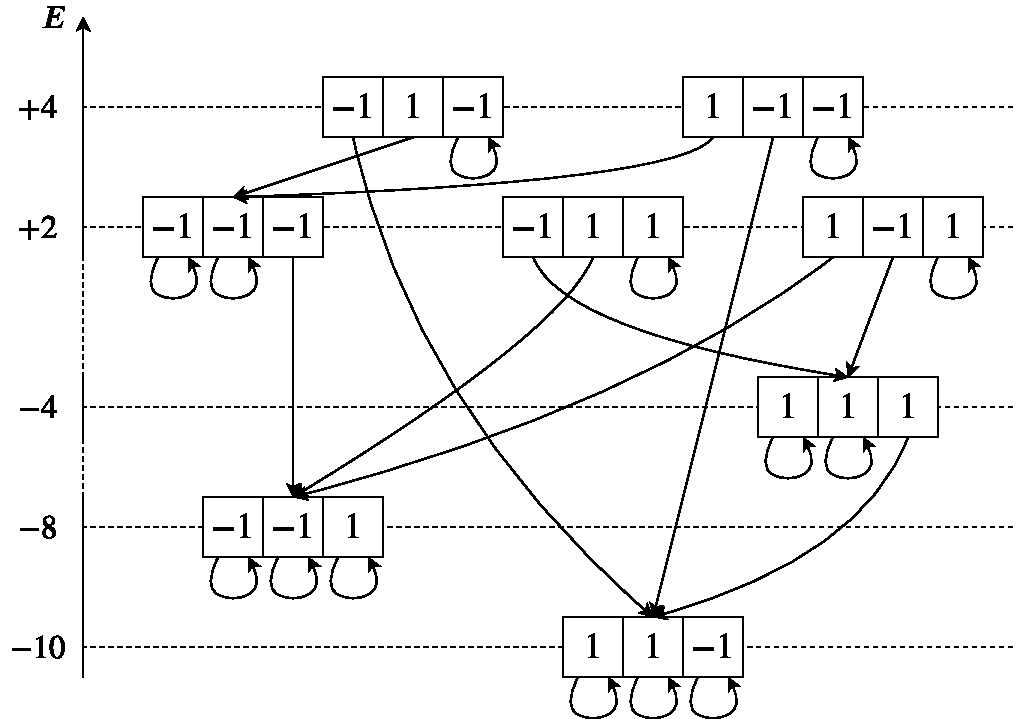
\includegraphics[width=0.7\linewidth]{async.pdf}
    \caption{State transition diagram with asynchronous update}
    \label{async}
\end{figure}

With respect to the synchronous case, it is possible to notice that this state transition model does not present any form of instability. In this case, there are no \emph{urstates} (each state has at least itself as a predecessor), while the \emph{stable states} of the network are unchanged, $[\begin{matrix} -1 & -1 & +1 \end{matrix}]^T$ and $[\begin{matrix} +1 & +1 & -1 \end{matrix}]^T$ (they have no successor states, excluding themselves).

\end{document}